\documentclass[twoside]{article}
\usepackage{fullpage}
\usepackage[utf8]{inputenc}
\usepackage{multicol}
\usepackage{amsmath}
\usepackage{float}
\usepackage{epsfig,graphicx}
\usepackage{xcolor,import}
\usepackage{caption}
\usepackage{subcaption}
\usepackage[font=small,labelfont=bf]{caption}
\usepackage{siunitx}
\usepackage[german]{babel}
\usepackage{textcomp}
\usepackage{mathtools}
\usepackage{subcaption}
\usepackage{cleveref}

\begin{document}


\thispagestyle{empty}
			\begin{center}
			\Large{Fakultät für Physik}\\
			\end{center}
\begin{verbatim}


\end{verbatim}
							%Eintrag des Wintersemesters
			\begin{center}
			\textbf{\LARGE SOMMERSEMESTER 2015}
			\end{center}
\begin{verbatim}


\end{verbatim}
			\begin{center}
			\textbf{\LARGE{Physikalisches Praktikum II}}
			\end{center}
\begin{verbatim}




\end{verbatim}

			\begin{center}
			\textbf{\LARGE{PROTOKOLL}}
			\end{center}
			
\begin{verbatim}





\end{verbatim}

			\begin{flushleft}
			\textbf{\Large{Experiment Nr.5: Polarisation}}\\
							%Experiment Nr. und Titel statt den Punkten eintragen
			\LARGE{}	
			\end{flushleft}

\begin{verbatim}

\end{verbatim}	
							%Eintragen des Abgabedatums, oder des Erstelldatums des Protokolls
			\begin{flushleft}
			\textbf{\Large{Datum:}} \Large{24.04.2015}
			\end{flushleft}
			
\begin{verbatim}
\end{verbatim}
							%Namen der Protokollschreiber
		\begin{flushleft}
			\textbf{\Large{Bachleitner Veronika, Grafendorfer Erik}} 
			\end{flushleft}

\begin{verbatim}


\end{verbatim}
							%Kurstag und Gruppennummer, zb. Fr/5
			\begin{flushleft}
			\textbf{\Large{Kurstag/Gruppe:}} \Large{FR/1}
			\end{flushleft}

\begin{verbatim}






\end{verbatim}
							%Name des Betreuers, das Praktikum betreute.
			\begin{flushleft}
			\LARGE{\textbf{Betreuer:\Large{ KLEPP }}}		
			\end{flushleft}

\newpage
\section{Aufgabenstellung}
Wir untersuchen mittels polarisiertem Licht verschiedene Eigenschaften von Materialien, wie die Schwingungsrichtung der Dipole in einer Glasplatte, die den Brewsterwinkel vorgibt, die Spannungszustände in einer Plexiglasprobe unter Druck und die optische Aktivität von Quarz und einer Zuckerlösung.

\section{Theorie}
\subsection{Brewster Winkel}
Wenn Licht auf eine Glasplatte trifft und in ihr gebrochen wird, oszillieren die elektrischen Dipole in der Platte senkrecht auf die Ausbreitungsrichtung des gebrochenen Strahls. Wenn linear polarisiertes Licht nun so auf die Platte fällt, dass der Winkel eines an der Oberfläche reflektierten Strahles senkrecht auf den des gebrochenen Strahles stehen würde, kann kein Licht reflektiert werden, weil in der Richtung der Oszillation der Dipole, senkrecht auf den gebrochenen Strahl, keine Energie abgestrahlt werden kann. Diesen Einfallswinkel nennt man Brewsterwinkel.\\
\\
Die Formel 
$$\tan \alpha_B=\frac{n_2}{n_1}$$
gibt den Zusammenhang zwischen dem Brewsterwinkel und den Brechungsindizes der beiden Medien an.

\subsection{Spannungsoptik}

In der Spannungsoptik wird mithilfe von polarisiertem Licht die Spannungsverteilung in lichtdurchlässigen Körpern untersucht. Bei einem doppelbrechenden Material (optisch anisotrop) wird die Polarisationsebene des einfallenden Lichts gedreht. Wird nun der Körper verformt ändert sich das Licht beim Durchgang durch den Körper. Diese Veränderung wird in diesem Experiment beobachtet.\\
Die Hauptgleichung der Spannungsoptik ist:
$$\delta\frac{1}{S}(\sigma_1 - \sigma_2)d$$
wo $S=\lambda/C$ die Spannungsoptische Konstante, $\sigma_i$ die Hauptspannungen und $d$ die Dicke der Probe. \\
$\delta$ ist die Phasenverschiebung, die im Sinne einer Ordnungszahl angegeben wird: $\delta=0,1,2,...$\\
Es treten Isochromaten und Isoklinen auf. Die Isochromaten sind experimentell gefundene Linien gleicher Hauptspannungsdifferenz ($\sigma_1-\sigma_2$). Wenn die Hauptspannungen mit der Polarisationsrichtung zusammenfallen, sieht man Isoklinen.

\subsection{Optische Aktivität}
Durch gleichmäßigen Druck auf eine Probe aus Plexiglas lässt sich die Achse, in der der Druck wirkt, zur einen optischen Achse der Probe machen. Fällt auf diese Achse wird es in einen ordentlichen und einen außerordentlichen Strahl aufgespalten
Für den gemessenen Drehwinkel $\alpha$, den spezifischen Drehwinkel $[\alpha]$, die Zuckerkonzentration $C$ und die Durchtrittslänge $l$ gilt:
\begin{equation*}
\alpha=[\alpha]\cdot C \cdot l
\end{equation*} 
\begin{equation}
\label{eq:SpezDrehwinkel}
[\alpha]=\frac{\alpha}{ C \cdot l }
\end{equation} 
\section{Aufbau}
\subsection{Brewster Winkel}
Für das Experiment verwenden wir eine Lichtquelle, einen Polarisator (Glan-Thompson-Prisma), eine drehbare Planparallele Platte und einen drehbaren Photodetektor, mit dem die Intensität des reflektierten Lichtes über einen Photowiderstand an einem Ampéremeter abgelesen werden kann.\\
Die Polarisation des Lichts wird über die Drehung des Prismas eingestellt (Strichmarkierung).

\subsection{Spannungsoptik}

\subsection{Optische Aktivität}
Wir verwenden für die Messung des Drehsinns ein Halbschattenpolarimeter von Lippich und halten Ausschau nach der Abfolge der Farben \textbf{grün - blau - rot - gelb} bei Drehung des Analysators.\\
Für die Messung des spezifischen Drehwinkels einer Zuckerlösung verwenden wir ein Polarimeter nach Laurent der Fa. Krüss.
\section{Durchführung}
\subsection{Brewster Winkel}
\subsection{Spannungsoptik}
\subsection{Optische Aktivität}

\section{Ergebnisse}
\subsection{Brewster Winkel}
Aus dem gemessenen Winkel $\delta$ ergibt sich der Einfallswinkel $\alpha=\frac{180-\delta}{2}$.\\
Ohne Platte sehen wir die maximale Intensität von $1.41 \si{mA}$ bei $-0^\circ20'$. Da wir im Folgenden gar nicht so exakt messen ($\pm 50'$), kann dieser Offset vernachlässigt werden.\\
\\
Die Messung ergibt schließlich folgende Werte:

\begin{table}[H]
\begin{center}
\begin{tabular}{|c|c|c|c|}
\hline
$\alpha$ ($^\circ, \pm 50'$) & $\delta$ ($^\circ, \pm 50'$) & $I_1$ ($\si{mA}$) & $I_2$ ($\si{mA}$)\\
\hline
35 & 110 & 0.114 & 0.045\\
40 & 100 & 0.132 & 0.037\\
45 & 90 & 0.162 & 0.027\\
50 & 80 & 0.192 & 0.019\\
55 & 70 & 0.228 & 0.0132\\
60 & 60 & 0.285 & 0.0183\\
65 & 50 & 0.370 & 0.041\\
\hline
\end{tabular}
\end{center}
\end{table}
\vspace{0.5mm}

Wobei die Unsicherheit der Intensitäten immer $\pm$ die letzte angegebene Stelle ist. Leider haben wir keine Zwischenwerte nahe des Minimums gemessen.

\begin{center}
\begin{figure}[H]
\begin{subfigure}{0.52\textwidth}
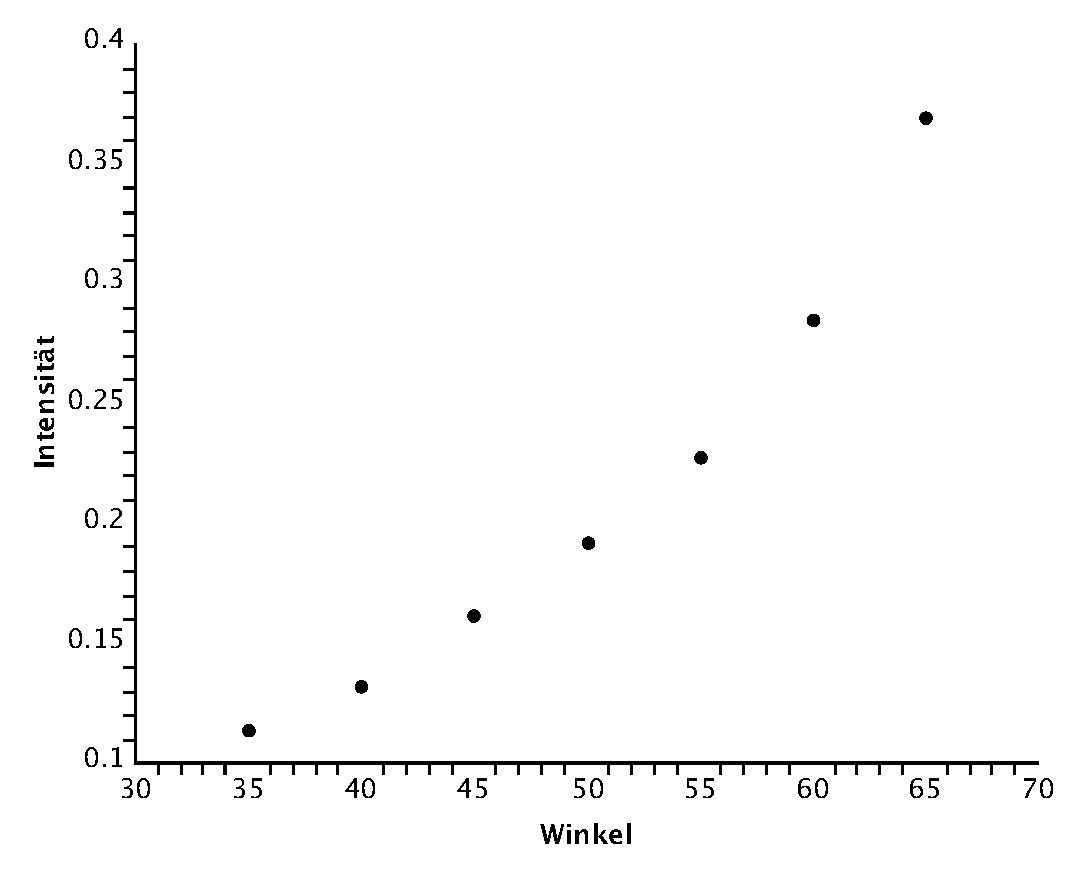
\includegraphics[width=0.9\linewidth]{reflexion_senkrecht.eps}
\caption{}
\end{subfigure}
\begin{subfigure}{0.52\textwidth}
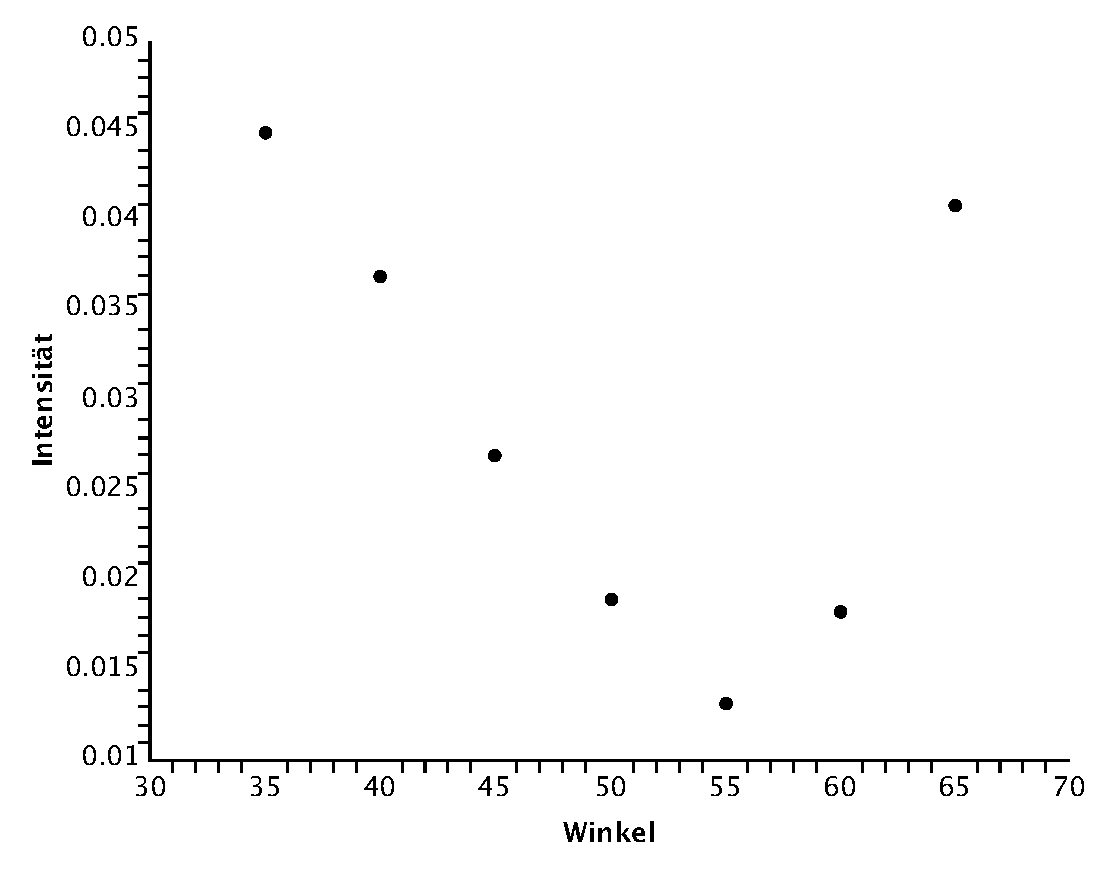
\includegraphics[width=0.9\linewidth]{reflexion_parallel.eps}
\caption{}
\end{subfigure}
\caption{Die Intensität des reflektierten Lichts als Funktion des Winkels für senkrecht (a) und parallel (b) zur Einfallsebene polarisiertes Licht.}
\end{figure}
\label{fig:brewster}
\end{center}

Aus Abbildung \ref{fig:brewster} kann der Brewster-Winkel mittels Augenmaß als das Minimum in (b) bestimmt werden.
$$\boxed{\alpha_B=(56 \pm 1)^\circ}$$
Die Unsicherheit wird aufgrund der Methode so gewählt.
Aus dem Brewster Winkel ergibt sich mit $\tan \alpha_B=\frac{n_2}{n_1}$ und dem Brechungsindex der Luft $n_1 \approx 1$ der Brechungsindex der Platte. Die Unsicherheit dazu wird mithilfe der Größtfehlerabschätzung angegeben.
$$\boxed{n_2=\tan \alpha_B=1.48 \pm 0.05}$$

%\begin{table}
%\begin{center}
%\begin{tabular}{|c|c|c|c|}
%\hline
%$\alpha$ & $\delta$ & $I_1$ & $I_2$\\
%\hline
%35 & 110 & 38 bei 0.3 & 45 bei 0.1 -> 0.045
%40 & 100 & 44 & 37 bei 0.1 -> 0.037
%45 & 90 & 54 & 27 
%50 & 80 & 64 & 19
%55 & 70 & 76 & 44 bei 0.03 -> 0.0044*3=0.0132
%60 & 60 & 95 und 29 bei 1 & 61 bei 0.03 bzw. 20 bei 0.1
%65 & 50 & 37 bei 1 & 41 bei 0.1
%\hline
%\end{tabular}
%\end{center}
%\end{table}


\subsection{Spannungsoptik}
Durchmesser $a=7.5cm$, also Fläche: $A=(a/2)^2\pi=441.7mm^2$\\
Dicke der Probe: $d=10.3mm$\\
Querschnittsfläche: $10.3mm^2=106.09mm^2$\\
$1 bar = 0.1 N/mm^2$\\
$S=\frac{\sigma d}{\delta}$\\
$\lambda=590nm$\\
$C_=\frac{\lambda}{S}$\\
\\
\begin{table}[H]
\begin{center}
\begin{tabular}{|c|c|c|c|c|r|}
\hline
$n$ & $p$ ($\pm 0.5$, bar) & $p$ ($\pm 0.05$, $\si{N/mm^2}$) & $F$ ($N$) & $\sigma$ ($\si{N/mm^2}$) & $S$ ($\si{N/mm}$)\\
\hline
1 & 2.0 & 0.20 & 883.12 & 8.3243 & $86 \pm 22$\\
2 & 5.5 & 0.55 & 2428.59 & 22.8918 & $118 \pm 11$\\
3 & 9.0 & 0.90 & 3974.06 & 37.4594 & $128.6 \pm 7.2$\\
4 & 12.0 & 1.20 & 5298.75 & 49.9458 & $128.6 \pm 5.4$\\
5 & 15.5 & 1.55 & 6844.22 & 64.5133 & $132.9 \pm 4.3$\\
\hline
\end{tabular}
\end{center}
\end{table}
\vspace{0.5mm}

Da die Unsicherheiten der Querschnittsfläche und Dicke der Probe im Vergleich zur Unsicherheit der Druckmessung gering ist, vernachlässigen wir diese. Wir geben die Unsicherheiten zu den Zwischenschritten ($F$, $\sigma$) nicht an, sondern schließen mittels der relativen Unsicherheit der Druckmessung direkt auf die Unsicherheit von $S$.\\
Diese Unsicherheit ist dann gegeben durch $\frac{\Delta p}{p} \cdot S$, zum Beispiel Ordnung 2: $\frac{0.5}{5.5} \cdot 117.89=10.72 \Rightarrow S=(118 \pm 11) \si{N/mm}$.\\
\\
Der Mittelwert für $S$ aus allen 5 Ordnungen und daraus $C$ ist
$$S=(119 \pm 19)\si{N/mm} \Rightarrow C=(4.97 \pm 0.79) \cdot 10^{-6}\si{mm^2/N}$$
\\
Der Mittelwert für $S$ aus den Ordnungen 2 bis 5 und daraus $C$ ist
$$\boxed{S=(127.0 \pm 6.4)\si{N/mm} \Rightarrow C=(4.64 \pm 0.24) \cdot 10^{-6}\si{mm^2/N}}$$

\subsection{Optische Aktivität}
Wenn die Ausbreitungsrichtung des Lichtes als positive Koordinatenrichtung gewählt wird, drehten 2 der Quarzproben im mathematisch positiven Sinn, also linksdrehend, und eine im mathematisch negativen Sinn, also rechtsdrehend.\\
Wir vermischten $(2.0 \pm 0.1)$ g Zucker mit $(20 \pm 1)\text{ml} \approx (20 \pm 1)$ g Wasser. Das ergibt die Konzentration:
$$C=\frac{(2.0 \pm 0.1) \text{g Zucker}}{(20 \pm 1) \text{g Wasser}}$$
$$\Delta C= \sqrt{\frac{\Delta Zucker^2}{Wasser^2}+\frac{Zucker^2 \cdot \Delta Wasser^2}{Wasser^4}} = \sqrt{\frac{0.1^2}{20^2}+\frac{4}{20^4}}\approx 0.01$$
\vspace{0.5cm}
$$C=(0.1\pm0.01)$$
Die Zuckerlösung drehte das Licht um $13^\circ 6' \pm 3'$, und zwar in mathematisch negativem Sinn. \\
Daraus, und mit der Länge $l$=2dm, schließen wir mit der Gleichung (\ref{eq:SpezDrehwinkel}) und der Unsicherheit:
$$\Delta [\alpha] = \sqrt{\frac{\Delta \alpha^2}{l^2\cdot C^2}+\frac{\alpha^2 \cdot \Delta C ^2}{l^2\cdot C^4}}$$
$$\Delta [\alpha] = \sqrt{\frac{0.5^2}{4\cdot 0.1^2}+\frac{13.1^2\cdot 0.01^2}{4 \cdot 0.1^4}}$$
$$\Delta [\alpha] \approx 7.1 \frac{^\circ}{dm}$$

\begin{center}
\fbox{$[\alpha] = (65.5 \pm 7.1)\frac{^\circ}{dm}$}
\end{center}
\section{Diskussion}
\subsection{Brewster Winkel}
\subsection{Spannungsoptik}

Der Mittelwert aller fünf Messwerte ist $S=(119 \pm 19)\si{N/mm}$. Vernachlässigen wir allerdings den Wert bei der 1. Ordnung erhalten wir $S=(127.0 \pm 6.4)\si{N/mm}$; dieser Wert liegt sehr gut innerhalb der 1$\sigma$ Vertrauensbereiche der anderen Messwerte! Darum gehen wir davon aus dass die Messung bei der 1. Ordnung nicht genau war, eine Feststellung, die weiter davon bestärkt wird dass in einer zweiten Messung ein Wert von $2.5 \si{bar}$ gemessen wurde.\\
Bedenken wir zusätzlich, dass wir eine Unsicherheit von $0.5 \si{bar}$ für die Messung des Drucks annehmen, bedeutet das also, dass der Wert der 1. Ordnung eigentlich ($2.0 \pm 1.0)\si{bar}$ beträgt. Das ist bereits eine relative Unsicherheit von 50\%, wodurch auch dieser Messwert innerhalb der Unsicherheitsgrenzen liegt. 

\subsection{Optische Aktivität}
																					
\end{document}
